\documentclass{article}

\usepackage{graphicx}
\usepackage{tikz}
\usepackage{tikzsymbols}
\usetikzlibrary{calc,patterns,shapes.geometric}
\pagestyle{empty}
\usepackage[margin=0pt]{geometry}
\geometry{papersize={14in,12in}}

\def\centerarc[#1](#2)(#3:#4:#5){\draw[#1] ($(#2)+({#5*cos(#3)},{#5*sin(#3)})$) arc (#3:#4:#5);}

\begin{document}
	\begin{figure}
		\centering
		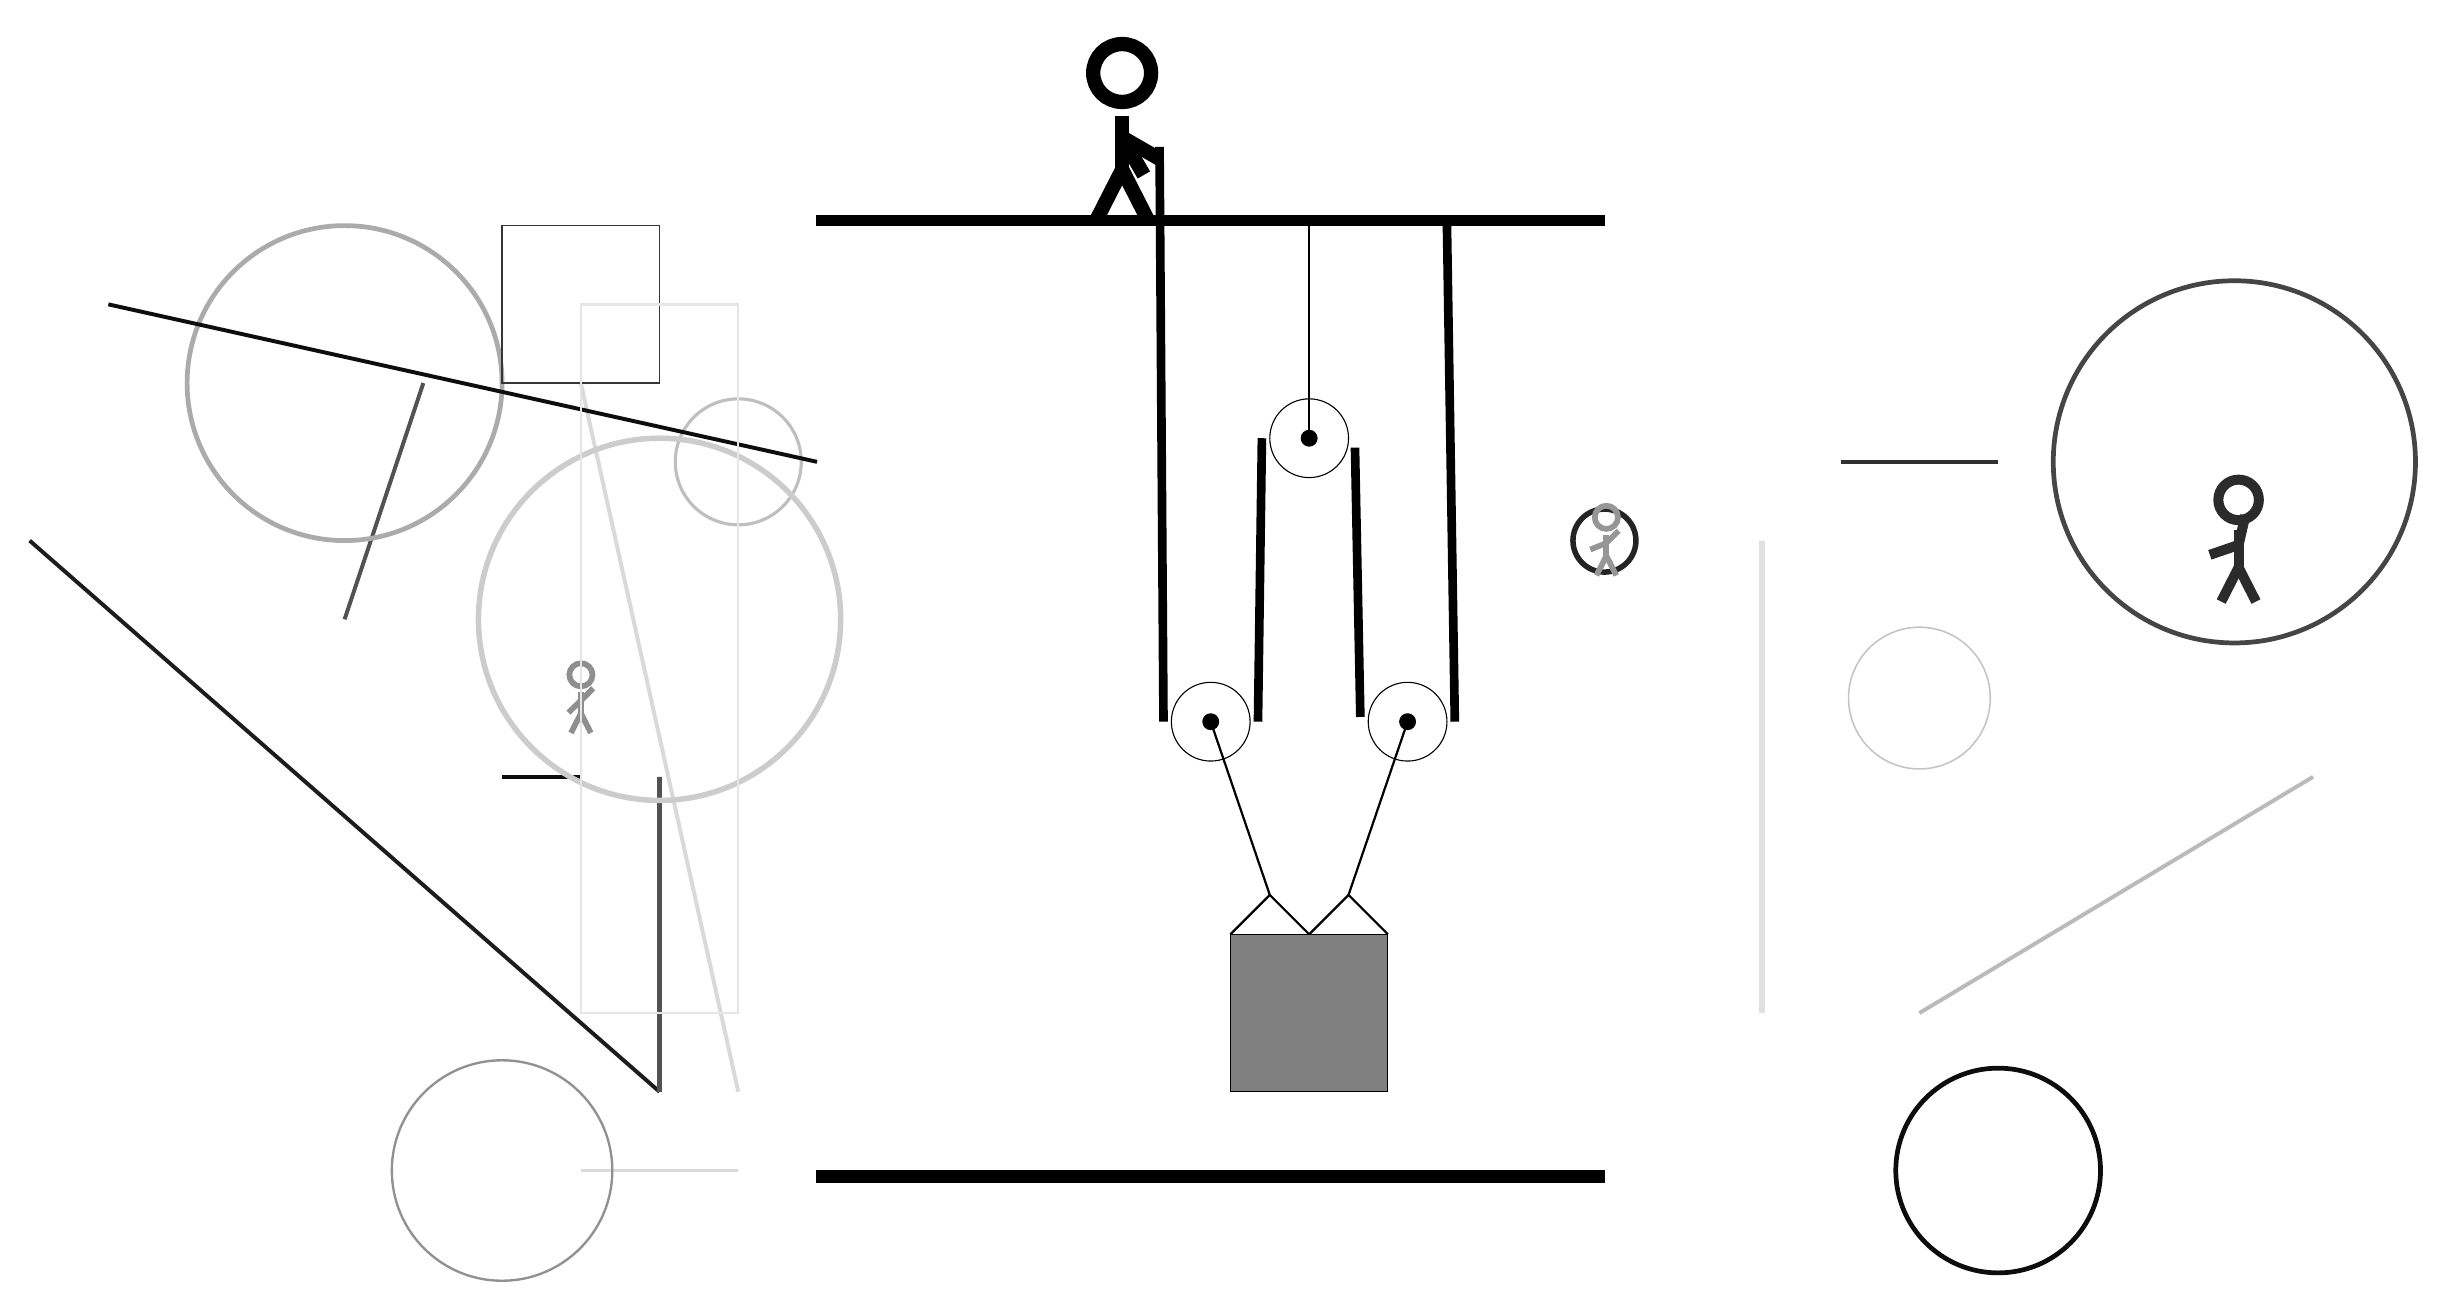
\begin{tikzpicture}
			%%%%% START %%%%%
			
			\draw[fill=black] (-4, 9) rectangle (6, 9.125);
			
			\draw (1, 2.7) circle (0.5);
			\draw[fill=black] (1, 2.7) circle (0.1);
			
			\draw (2.25, 6.3) circle (0.5);
			\draw[fill=black] (2.25, 6.3) circle (0.1);
			\draw[thick] (2.25, 6.3) -- (2.25, 9);
			
			\draw (3.5, 2.7) circle (0.5);
			\draw[fill=black] (3.5, 2.7) circle (0.1);
			
			\draw[thick] (3.5, 2.7) -- (2.75, 0.5);
			\draw[thick] (1, 2.7) -- (1.75, 0.5);
			\draw[thick]  (1.25, 0) -- (1.75, 0.5) -- (2.25, 0);
			\draw[thick]  (2.25, 0) -- (2.75, 0.5) -- (3.25, 0);
			\draw[fill=black!50] (1.25, 0) rectangle (3.25, -2);
			
			\draw[line width=1.1mm] (0.35, 10) --  (0.4, 2.7);
			\centerarc[line width=1.1mm](1, 2.7)(180:360:0.6);
			\draw[line width=1.1mm] (1.6, 2.7) -- (1.65, 6.3);
			\centerarc[line width=1.1mm](2.25, 6.3)(-20:180:0.6);
			\draw[line width=1.1mm](2.832, 6.18) -- (2.9, 2.76);
			\centerarc[line width=1.1mm](3.5, 2.7)(160:360:0.6);
			\draw[line width=1.1mm](4.1, 2.7) -- (4.0, 9);
			
			\draw [line width=0.2mm, color=black!23](10, 3) circle (0.9);
			
			\draw [line width=0.6mm, color=black!95](11, -3) circle (1.3);
			\draw[line width=0.5mm, color=black!14] (-5, -3) rectangle (-7, -3);
			\draw[line width=0.5mm, color=black!15](-5, -2) -- (-7, 7);
			\draw[line width=0.5mm, color=black!89](-6, -2) -- (-14, 5);
			\draw[line width=0.7mm, color=black!12] (8, 5) rectangle (8, -1);
			\draw [line width=0.4mm, color=black!25](-5, 6) circle (0.8);
			\draw [line width=0.7mm, color=black!86](6, 5) circle (0.4);
			\node[line width=0.6mm, color=black!83] at (14, 5) {\Strichmaxerl[7][19][77]};
			\draw[line width=0.5mm, color=black!95](-7, 2) -- (-8, 2);
			\draw[line width=0.5mm, color=black!68](-9, 7) -- (-10, 4);
			\draw [line width=0.6mm, color=black!33](-10, 7) circle (2.0);
			\draw[line width=0.2mm, color=black!79] (-6, 9) rectangle (-8, 7);
			
			\node[line width=0.6mm, color=black!44] at (-7, 3) {\Strichmaxerl[4][44][45]};
			\draw[line width=0.6mm, color=black!68] (-6, -2) rectangle (-6, 2);
			\draw [line width=0.6mm, color=black!73](14, 6) circle (2.3);
			\draw[line width=0.5mm, color=black!27](10, -1) -- (15, 2);
			\draw[line width=0.5mm, color=black!29](-9, 5) -- (-9, 5);
			\draw[line width=0.5mm, color=black!81](11, 6) -- (9, 6);
			
			\draw [line width=0.7mm, color=black!20](-6, 4) circle (2.3);
			\draw[line width=0.5mm, color=black!95](-4, 6) -- (-13, 8);
			
			\draw [line width=0.3mm, color=black!43](-8, -3) circle (1.4);
			
			\node[line width=0.6mm, color=black!41] at (6, 5) {\Strichmaxerl[4][22][45]};
			\draw[line width=0.3mm, color=black!10] (-5, -1) rectangle (-7, 8);
			
			\node at (-0.07, 10.2) {\Strichmaxerl[10][120][-30]};
			
			\draw[fill=black] (-4, -3) rectangle (6, -3.15);
			
			%%%%% END %%%%%
		\end{tikzpicture}
	\end{figure}	
\end{document}